\documentclass[a4paper]{article}
\usepackage[utf8]{inputenc}
\usepackage[russian,english]{babel}
\usepackage[T2A]{fontenc}
\usepackage[left=10mm, top=20mm, right=18mm, bottom=15mm, footskip=10mm]{geometry}
\usepackage{indentfirst}
\usepackage{amsmath,amssymb}
\usepackage[italicdiff]{physics}
\usepackage{graphicx}
\graphicspath{{images/}}
\DeclareGraphicsExtensions{.pdf,.png,.jpg}
\usepackage{wrapfig}

\usepackage{caption}
\captionsetup[figure]{name=Рисунок}
\captionsetup[table]{name=Таблица}
  
\title{\underline{Отчет о выполненой лабораторной работе 1.2.1}}
\author{Антон Хмельницкий, Б01-306}

\begin{document}

\maketitle
\begin{center}
\Large{\textbf{Определение скорости полета пули при помощи баллистического маятника}}
\end{center}

\section{Аннотация}
    \par \textbf{Цель работы:} Определить скорость полёта пули применяя законы сохранения и использую баллистические маятники.\\
    \par \noindent \textbf{В работе используются:} Духовое ружьё на штативе, осветитель, оптическая система для измерения отклонений маятника, измерительная линейка, пули и весы для их взвешивания, баллистические маятники.

\section{Метод баллистического маятнкиа}

\subsection{Теоретические сведения}
При контакте пули с цилиндром можно записать ЗСИ:
	\begin{equation}
		 mu = (M+m)V
	\end{equation}
	где $m$ -- масса пули, $u$ -- скорость пули перед ударом, $V$-скорость цилиндра вместе с пулей после удара.
	\begin{equation}
		u=\frac{M+m}{m}V \approx \frac{M}{m}V \;\;\;\;\; V^2=2gh \;\;\;\;\; h = L(1-cos \varphi ) = 2L^2 sin \frac{\varphi^2}{2} \;\;\;\;\;\;\; \varphi \approx \frac{\Delta x}{L} 
	\end{equation}
        где $\varphi$ - угол отклонения маятника от вертикали, $\Delta x$ - отклонение маятника\\
	Тогда скорость пули можно выразить как
	\begin{equation} \label{vel1}
	 u=\frac{M}{m} \sqrt{\frac{g}{L}} \Delta x
	\end{equation}
\newpage
\subsection{Экспериментальная установка}
При попадании пули в цилиндр любая его точка движется по окружности известного радиуса, поэтому его смещение с помощью собирающей линзы можно перевести в линейное отклонение на линейке.\\
	\begin{figure}[!h]
		\begin{center}
			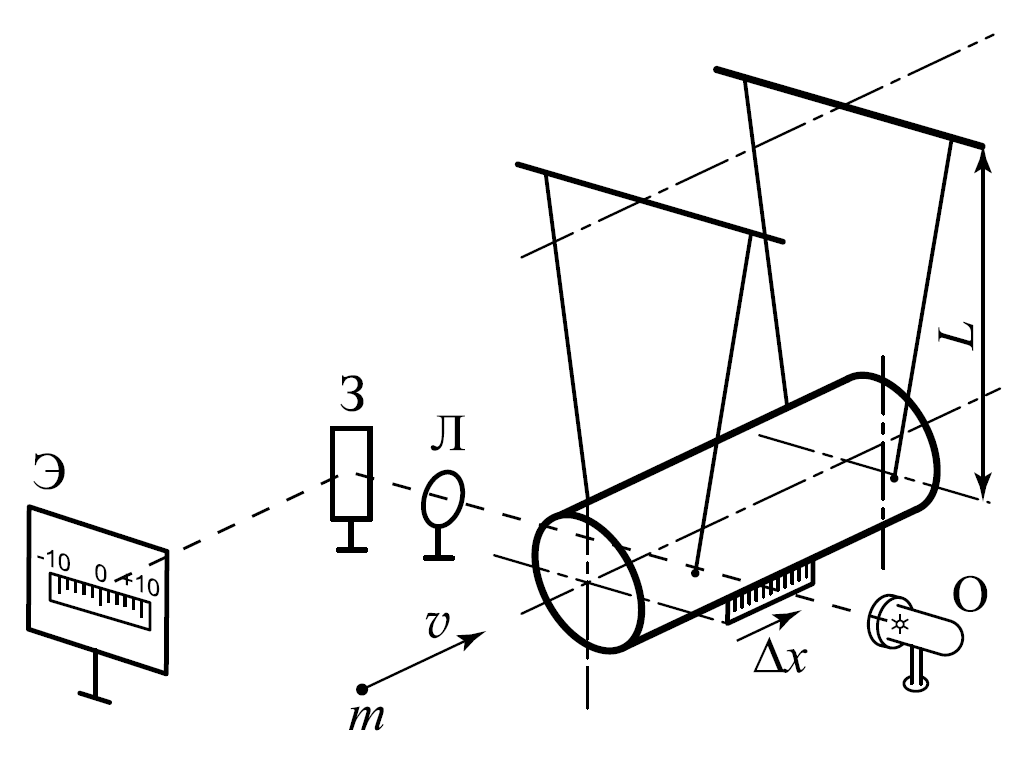
\includegraphics[scale = 0.8]{ustan1}
			\caption{схема установки для измерения скорости полета пули}
		\end{center}
	\end{figure}
\newpage
\subsection{Расчет всех данных}


\begin{table}[h!]
\begin{center}
\begin{tabular}{|c|c|}
\hline
Номер пули & Масса, гр \\ \hline
1          & 0,5086    \\ \hline
2          & 0,4955    \\ \hline
3          & 0,5031    \\ \hline
4          & 0,4998    \\ \hline
5          & 0,515     \\ \hline
6          & 0,5089    \\ \hline
7          & 0,5113    \\ \hline
8          & 0,5103    \\ \hline
9          & 0,5142    \\ \hline
10         & 0,5072    \\ \hline
\end{tabular}
\caption{Измерения масс пулей}
\end{center}
\end{table}

\begin{table}[h!]
\begin{center}
\begin{tabular}{|c|c|c|}
\hline
Расстояние от точки подвеса, $L$ & 222 см  & $\pm 0,5$ \\ \hline
Масса цилиндра, $M$              & 2925 гр & $\pm 5$   \\ \hline
\end{tabular}
\caption{Измерения параметров установки}
\end{center}
\end{table}

\begin{table}[h!]
\begin{center}
\begin{tabular}{|c|c|c|}
\hline
Номер пули & $x_{1}$, мм & $x_{2}$, мм \\ \hline
1          & 10      & 10      \\ \hline
2          & 9       & 8,5     \\ \hline
3          & 9       & 9,5     \\ \hline
4          & 9,4     & 9,4     \\ \hline
5          & 9,5     & 9,8     \\ \hline
\end{tabular}
\caption{Измерения отклонений при стрельбе}
\end{center}
\end{table}

\subsection{Обработка результатов}

Используя формулу:
\begin{equation} 
	 u=\frac{M}{m} \sqrt{\frac{g}{L}} \Delta x
\end{equation}
, где $\Delta x = \frac{x_{1}+x_{2}}{2}$, получаем такие данные

\begin{table}[h!]
\begin{center}
\begin{tabular}{|c|c|}
\hline
Номер пули & Скорость пули, м/с \\ \hline
1          & 120,8948           \\ \hline
2          & 108,5796           \\ \hline
3          & 113,0502           \\ \hline
4          & 115,642            \\ \hline
5          & 115,2137           \\ \hline
\end{tabular}
\caption{Расчетные скорости полета пули}
\end{center}
\end{table}

Средняя скорость получилась $\overline{u} = 114,7 м/с$
Погрешность:
\[
    \varepsilon_{u} = \sqrt{\left(\varepsilon_{M}\right)^2 + \left(\varepsilon_{m}\right)^2 + \left(\frac{1}{2}\varepsilon_{L}\right)^2 + \left(\varepsilon_{x}\right)^2}
\]
Получаем $\varepsilon_{u} = 1\%$. 
\begin{table}[h!]
\begin{center}
\begin{tabular}{|c|c|c|c|c|c|}
\hline
$\sigma_{M}$ & 0,5 гр & $M$ & 2925 гр   & $\varepsilon_{M}$ & $0,01\%$  \\ \hline
$\sigma_{m}$ & 0,0001 гр & $m$ & 0,5 гр   & $\varepsilon_{m}$ & $0,02\%$ \\ \hline
$\sigma_{L}$ & 0,5 см   & $L$ & 222 см    & $\varepsilon_{L}$ & $0,22\%$  \\ \hline
$\sigma_{x}$ & 0,05 мм  & $x$ & 5 мм & $\varepsilon_{x}$ & $1\%$ \\ \hline
\end{tabular}
\caption{Погрешности}
\end{center}
\end{table}

\section{Выводы}

В данной работе мы экспериментально определили скорость полета пули, как видно с высокой точностью. Отличия скоростей у разных пуль возникает из за во-первых их отличия по массе, а во вторых из-за параметров выстрела (аэродинамика и начальное положение в винтовке)

%=========================================================================
%=========================================================================
\newpage

\section{Метод баллистического маятнкиа}

\subsection{Теоретические сведения}
Считая удар неупругим, можно записать уравнение
	$$mur=I \Omega$$
	$r-$расстояние от линии полёта пули до оси вращения, $I$ -- момент инерции относительно этой оси, $\Omega$ -- угловая скорость маятника сразу после удара.
	
	Можно пренебречь затуханием колебаний и потерями энергии и записать ЗСЭ:
	$$ k \frac{\varphi^2}{2} = I \frac{\Omega^2}{2} $$
	\noindent где $k$ -- модуль кручения проволоки, $\varphi$ -- максимальный угол поворота маятника, тогда:
	\begin{equation} \label{vel2}
		 u = \varphi \frac{\sqrt{kI}}{mr} 
	\end{equation}
\begin{equation}
		\label{phi}
		\varphi \approx \frac{x}{d}
	\end{equation}
	
	где $x$ -- смещение изображения нити осветителя на шкале, которое легко можно измерить.
	
	Периоды колебаний маятника с грузами и без можно выразить как
	$$T_1= 2 \pi \sqrt{\frac{I - 2MR^2}{k}} \;\;\;\;\;\; T_2 = 2 \pi \sqrt{\frac{I}{k}}$$
	Тогда $\sqrt{kI}$ можно найти как:
	\begin{equation}
		\sqrt{kI} = \frac{4 \pi M R^2 T_2}{T_2^2 - T_1^2}
		\label{kl}
	\end{equation}
	$R$ -- расстояние от оси вращения до центров грузиков, $M$ - масса грузиков.
\newpage
\subsection{Экспериментальная установка}
Крутильный баллистический маятник.
	\begin{figure}[!h]
		\begin{center}
			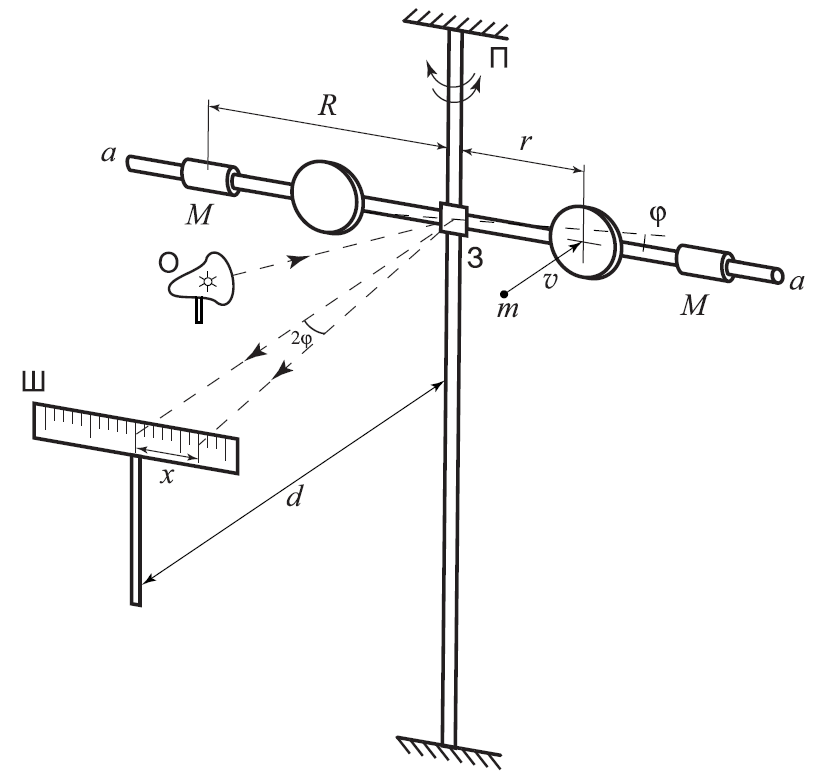
\includegraphics[scale = 0.8]{ustan2}
			\caption{схема установки для измерения скорости полета пули}
		\end{center}
	\end{figure}
\newpage
\subsection{Расчет всех данных}

\begin{table}[h!]
\begin{center}
\begin{tabular}{|c|c|c|c|}
\hline
Номер пули & $x_{1}$, см & $x_{2}$, см & Период, $T$, с \\ \hline
6          & 4,7     & 4,7     & 7,1         \\ \hline
7          & 4,5     & 4       & 6,94        \\ \hline
8          & 4,8     & 4,8     & 7           \\ \hline
9          & 4,1     & 4,1     & 6,97        \\ \hline
0          & 4,4     & 4,2     & 6,72        \\ \hline
\end{tabular}
\caption{Измерения отклонений и периода колебаний при стрельбе с грузами}
\end{center}
\end{table}

\begin{table}[h!]
\begin{center}
\begin{tabular}{|c|c|c|}
\hline
Расстояние до шкалы, $d$        & 125   & см \\ \hline
Расстояние от груза до оси, $R$ & 34    & см \\ \hline
Расстояние от пули до оси, $r$  & 22    & см \\ \hline
Масса груза 1, $M_{1}$             & 724,5 & гр \\ \hline
Масса груза 2, $M_{2}$             & 725,6 & гр \\ \hline
\end{tabular}
\caption{Параметры установки}
\end{center}
\end{table}

\begin{table}[h!]
\begin{center}
\begin{tabular}{|c|c|}
\hline
Номер измерения & Период колебаний, $T$,с \\ \hline
1               & 5,22                  \\ \hline
2               & 5,25                  \\ \hline
3               & 5,22                  \\ \hline
4               & 5,19                  \\ \hline
5               & 5,19                  \\ \hline
6               & 5,22                  \\ \hline
7               & 5,22                  \\ \hline
\end{tabular}
\caption{Период колебаний без грузов}
\end{center}
\end{table}

\subsection{Обработка результатов}

Для измеренных значений среднее будет $\overline{T_{1}} = 6,946 $ с и $\overline{T_{2}} = 5,22 $ с.\\
Для $T_{1}$:
\begin{itemize}
\item Среднее значение: $\langle T_{1} \rangle = \frac{1}{n}\sum\limits_{i=1}^n T_{1_i} = 6,946$ с. 
\item Стандартное отклонение: $\sigma_{T_{1}} = \sqrt{\frac{1}{n}\sum\limits_{i=1}^n(T_{1_i} - \langle T_{1} \rangle)^2} =  0.125$ с.
\item Стандартная погрешность опыта: $\sigma_\text{ср} = \frac{\sigma_{T_{1}}}{\sqrt{n}} =  0.05597$ с.
\item Полная погрешность: $\sigma_{\text{полн}} = \sqrt{\sigma_{\text{случ}}^2 + \sigma_{T_{1}}^2} = 0.0569$ с.
\end{itemize}
Для $T_{2}$:
\begin{itemize}
\item Среднее значение: $\langle T_{2} \rangle = \frac{1}{n}\sum\limits_{i=1}^n T_{2_i} = 5.2157$ с. 
\item Стандартное отклонение: $\sigma_{T_{2}} = \sqrt{\frac{1}{n}\sum\limits_{i=1}^n(T_{2_i} - \langle T_{2} \rangle)^2} = 0.0192$ с.
\item Стандартная погрешность опыта: $\sigma_\text{ср} = \frac{\sigma_{T_{2}}}{\sqrt{n}} =  0.0072$ с.
\item Полная погрешность: $\sigma_{\text{полн}} = \sqrt{\sigma_{\text{случ}}^2 + \sigma_{T_{2}}^2} = 0.0123$ с.
\end{itemize}
Итоговые результаты: \par

$T_{1} = 6,946 \pm 0,0569  (\varepsilon_{T_{1}} = 0,7\%)$ c\\
$T_{2} = 5,22 \pm 0,0123 (\varepsilon_{T_{2}} = 0,23\%)$ c\\

Тогда коэффициент $\sqrt{kI} = \frac{4 \pi M R^2 T_2}{T_2^2 - T_1^2} = 0,348$.\\

Погрешность:
\[
    \varepsilon_{\sqrt{kI}} = \sqrt{\left(\varepsilon_{M}\right)^2 + \left(2\varepsilon_{R}\right)^2 + \left(\frac{1}{2}\varepsilon_{T_{2}}\right)^2 + \left(\varepsilon_{T_{1}}\right)^2}
\]
Получаем $\varepsilon_{\sqrt{kI}} = 0,76\%$. 

\begin{table}[h!]
\begin{center}
\begin{tabular}{|c|c|c|c|c|c|}
\hline
$\sigma_{M}$ & 0,1 гр & $M$ & 725 гр   & $\varepsilon_{M}$ & $0,01\%$  \\ \hline
$\sigma_{R}$ & 0,5 мм & $R$ & 34 см   & $\varepsilon_{R}$ & $0,14\%$ \\ \hline
$\sigma_{T_{1}}$ & 0,0569 c & $T_{1}$ & 6,946 с    & $\varepsilon_{T_{1}}$ & $0,7\%$  \\ \hline
$\sigma_{T_{2}}$ & 0,0123 с  & $T_{2}$ &  5,22 с & $\varepsilon_{T_{2}}$ & $0,23\%$ \\ \hline
$\sigma_{m}$ & 0,0001 гр & $m$ & 0,5 гр   & $\varepsilon_{m}$ & $0,02\%$ \\ \hline
$\sigma_{x}$ & 0,5 мм  & $x$ & 5 см & $\varepsilon_{x}$ & $1\%$ \\ \hline
$\sigma_{d}$ & 0,5 мм  & $d$ & 125 см & $\varepsilon_{d}$ & $0,04\%$ \\ \hline
$\sigma_{r}$ & 0,05 мм  & $r$ & 22 см & $\varepsilon_{r}$ & $0,23\%$ \\ \hline
\end{tabular}
\caption{Погрешности}
\end{center}
\end{table}

Далее используя формулу $u = \frac{x}{d} \frac{\sqrt{kI}}{mr}$ получаем:
\begin{table}[h!]
\begin{center}
\begin{tabular}{|c|c|}
\hline
Номер пули & Скорость полета пули, $u$ \\ \hline
6          & 116,872                   \\ \hline
7          & 105,186                   \\ \hline
8          & 119,032                   \\ \hline
9          & 100,902                   \\ \hline
0          & 107,284                   \\ \hline
\end{tabular}
\caption{Скорости полета пули}
\end{center}
\end{table}

Средняя $\overline{u} = 109,86$ м/с
Погрешность:
\[
    \varepsilon_{u} = \sqrt{\left(\varepsilon_{x}\right)^2 + \left(\varepsilon_{d}\right)^2 + \left(\varepsilon_{\sqrt{kI}}\right)^2 + \left(\varepsilon_{m}\right)^2 + \left(\varepsilon_{r}\right)^2}
\]
Получаем $\varepsilon_{u} = 1,28\%$. 

\section{Выводы}

В данной работе мы экспериментально посчитали скорость полета пули. Отличия скоростей возникают из-за разных начальных прамаетров и аэродинамики.

\end{document}
